\newpage
\setcounter{chapter}{6}
\setcounter{section}{0}
\rsp \rsp \chapter*{Anexos: Planos de Ingeniería}\rsp\rsp
\addcontentsline{toc}{chapter}{{Anexos}} 
\addcontentsline{toc}{section}{{Planos de Ingeniería}} 

\section{Anexo 1. Vista explosionada de la cámara de refrigeración} 

\begin{minipage}{\textwidth} 
	\begin{figure}[H]
	\centering 
	\caption*{\textit{Continuación de anexo 4.}}\rsp\rsp\rsp\rsp
	\vspace{6cm}
	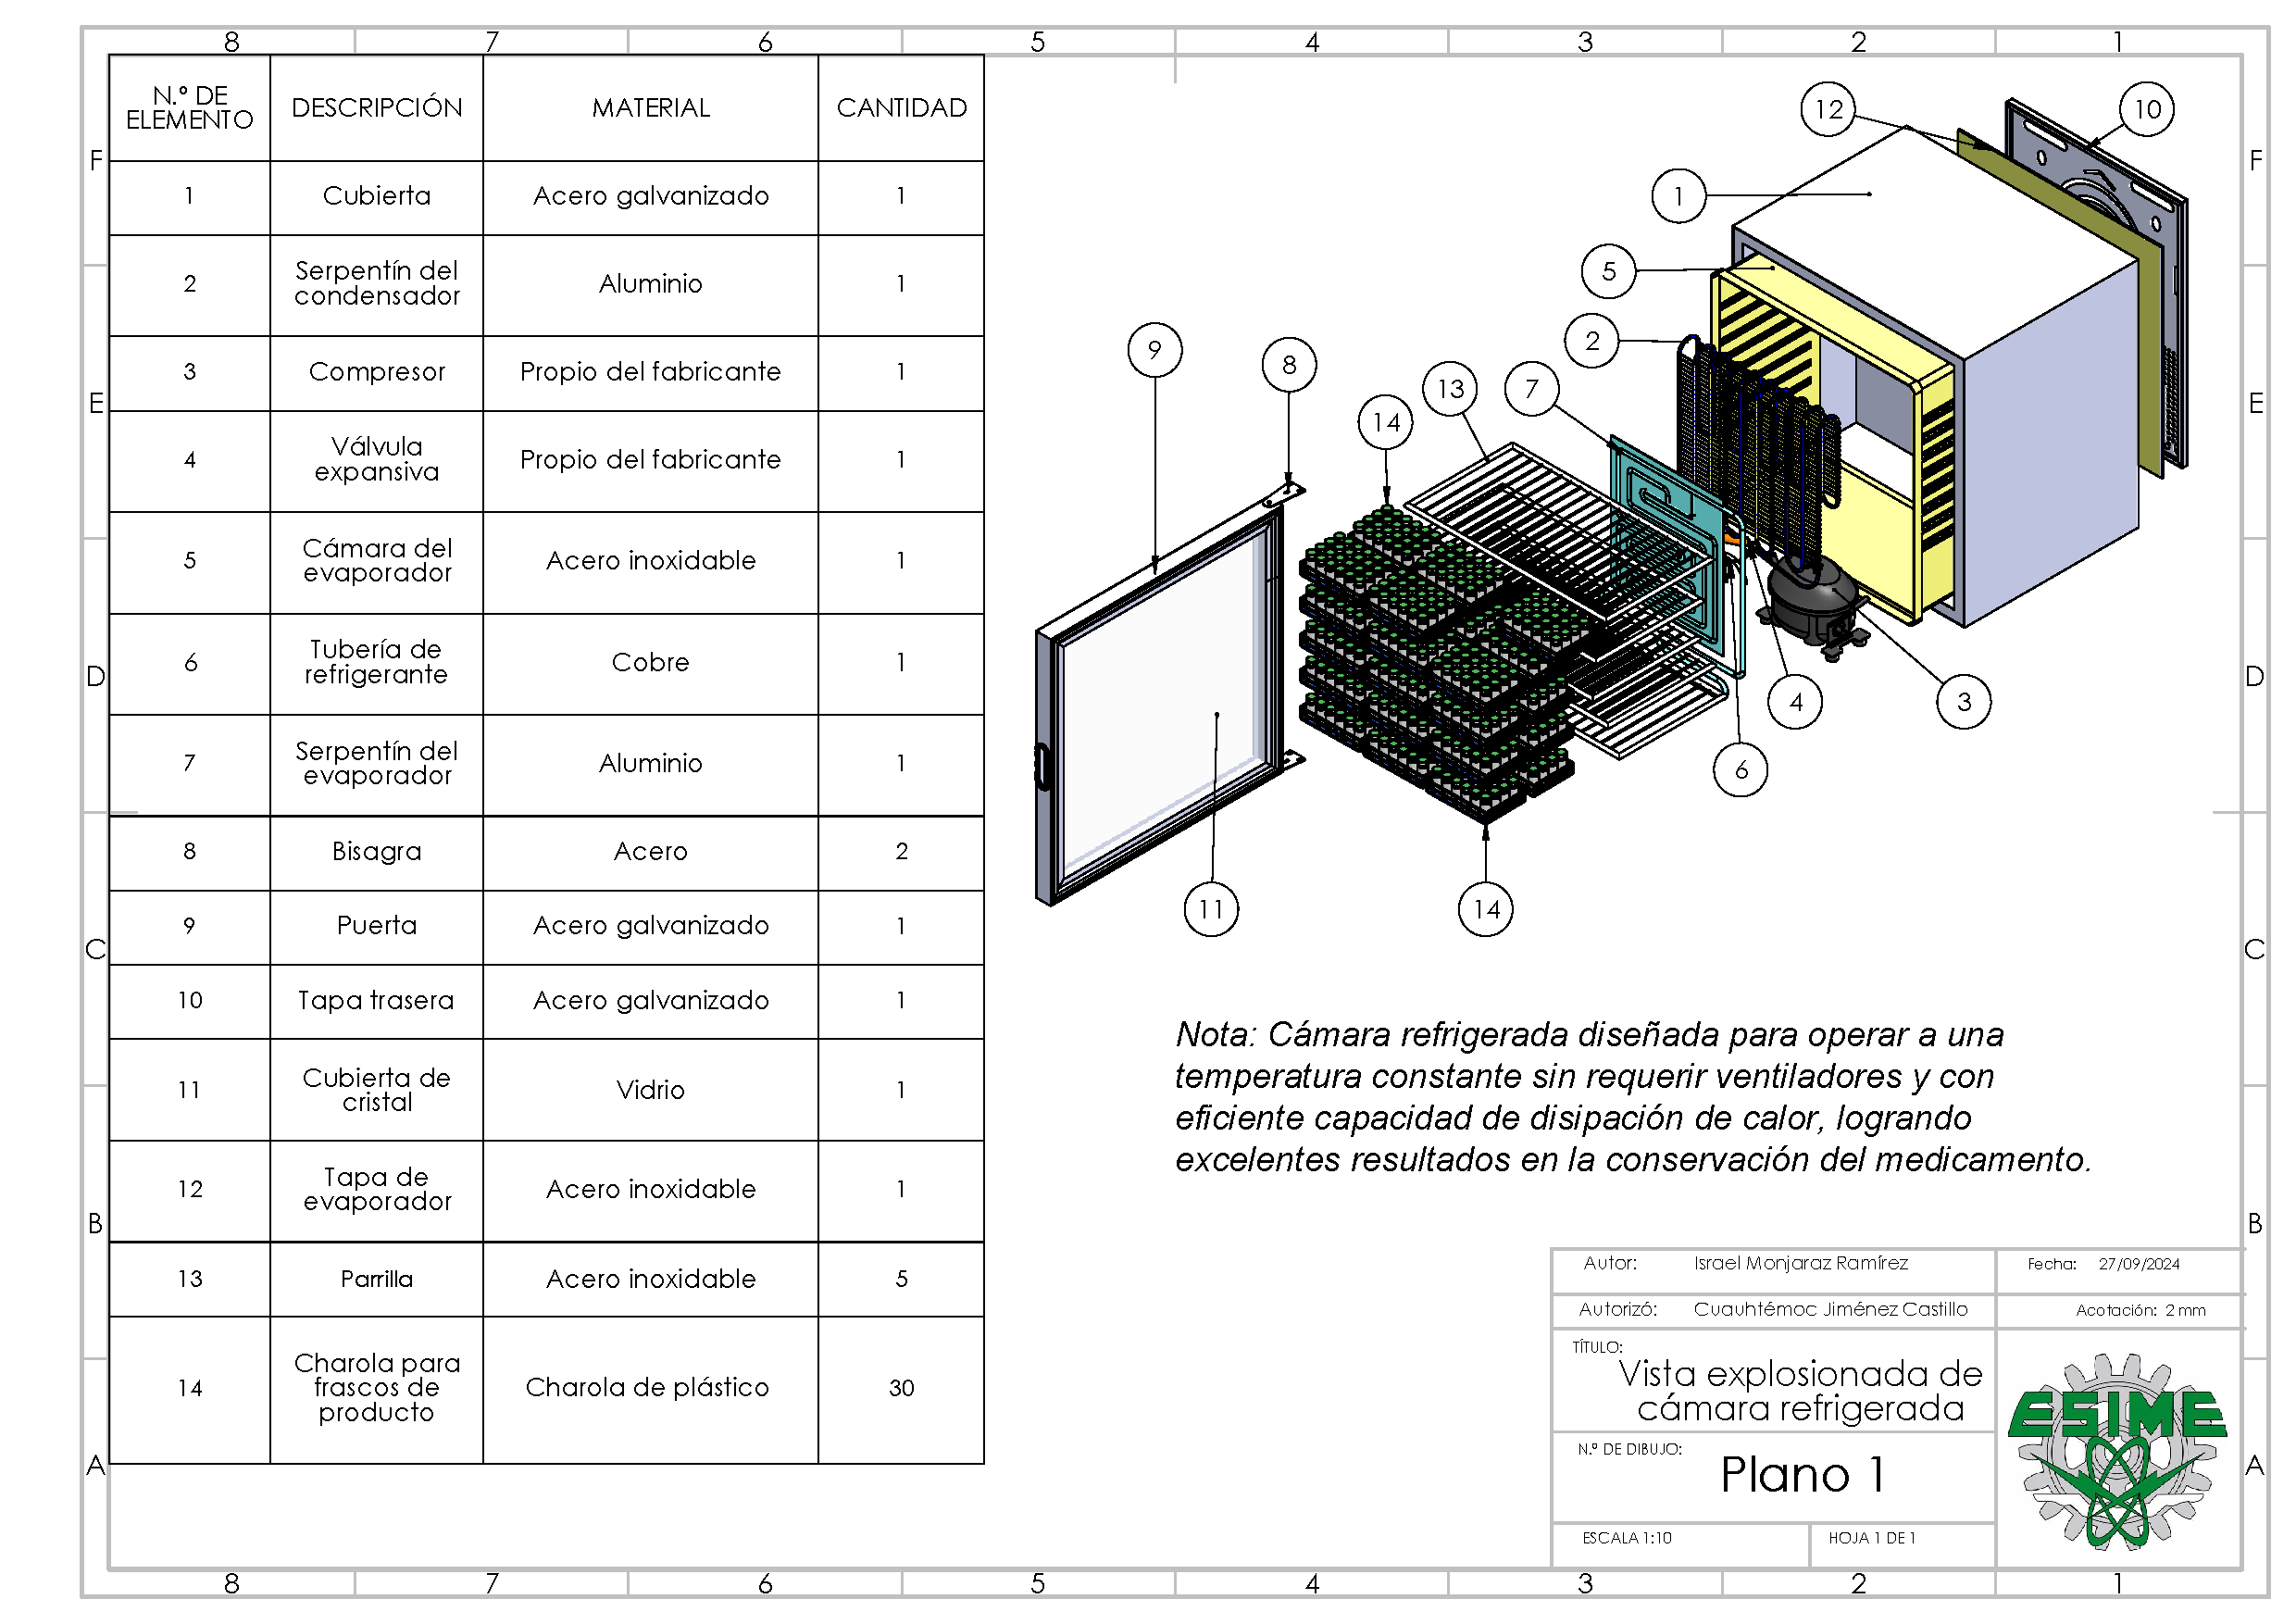
\includepdf[scale=0.75, angle=90]{pdfs/vista-explosionada.pdf}
	\label{axo:vista-explosionada}
\end{figure} 
\end{minipage}
\newpage
\section{Anexo 2. Cuatro vistas de la cámara de refrigeración} 
\begin{minipage}{\textwidth} 
	\begin{figure}[H]
		\centering 
		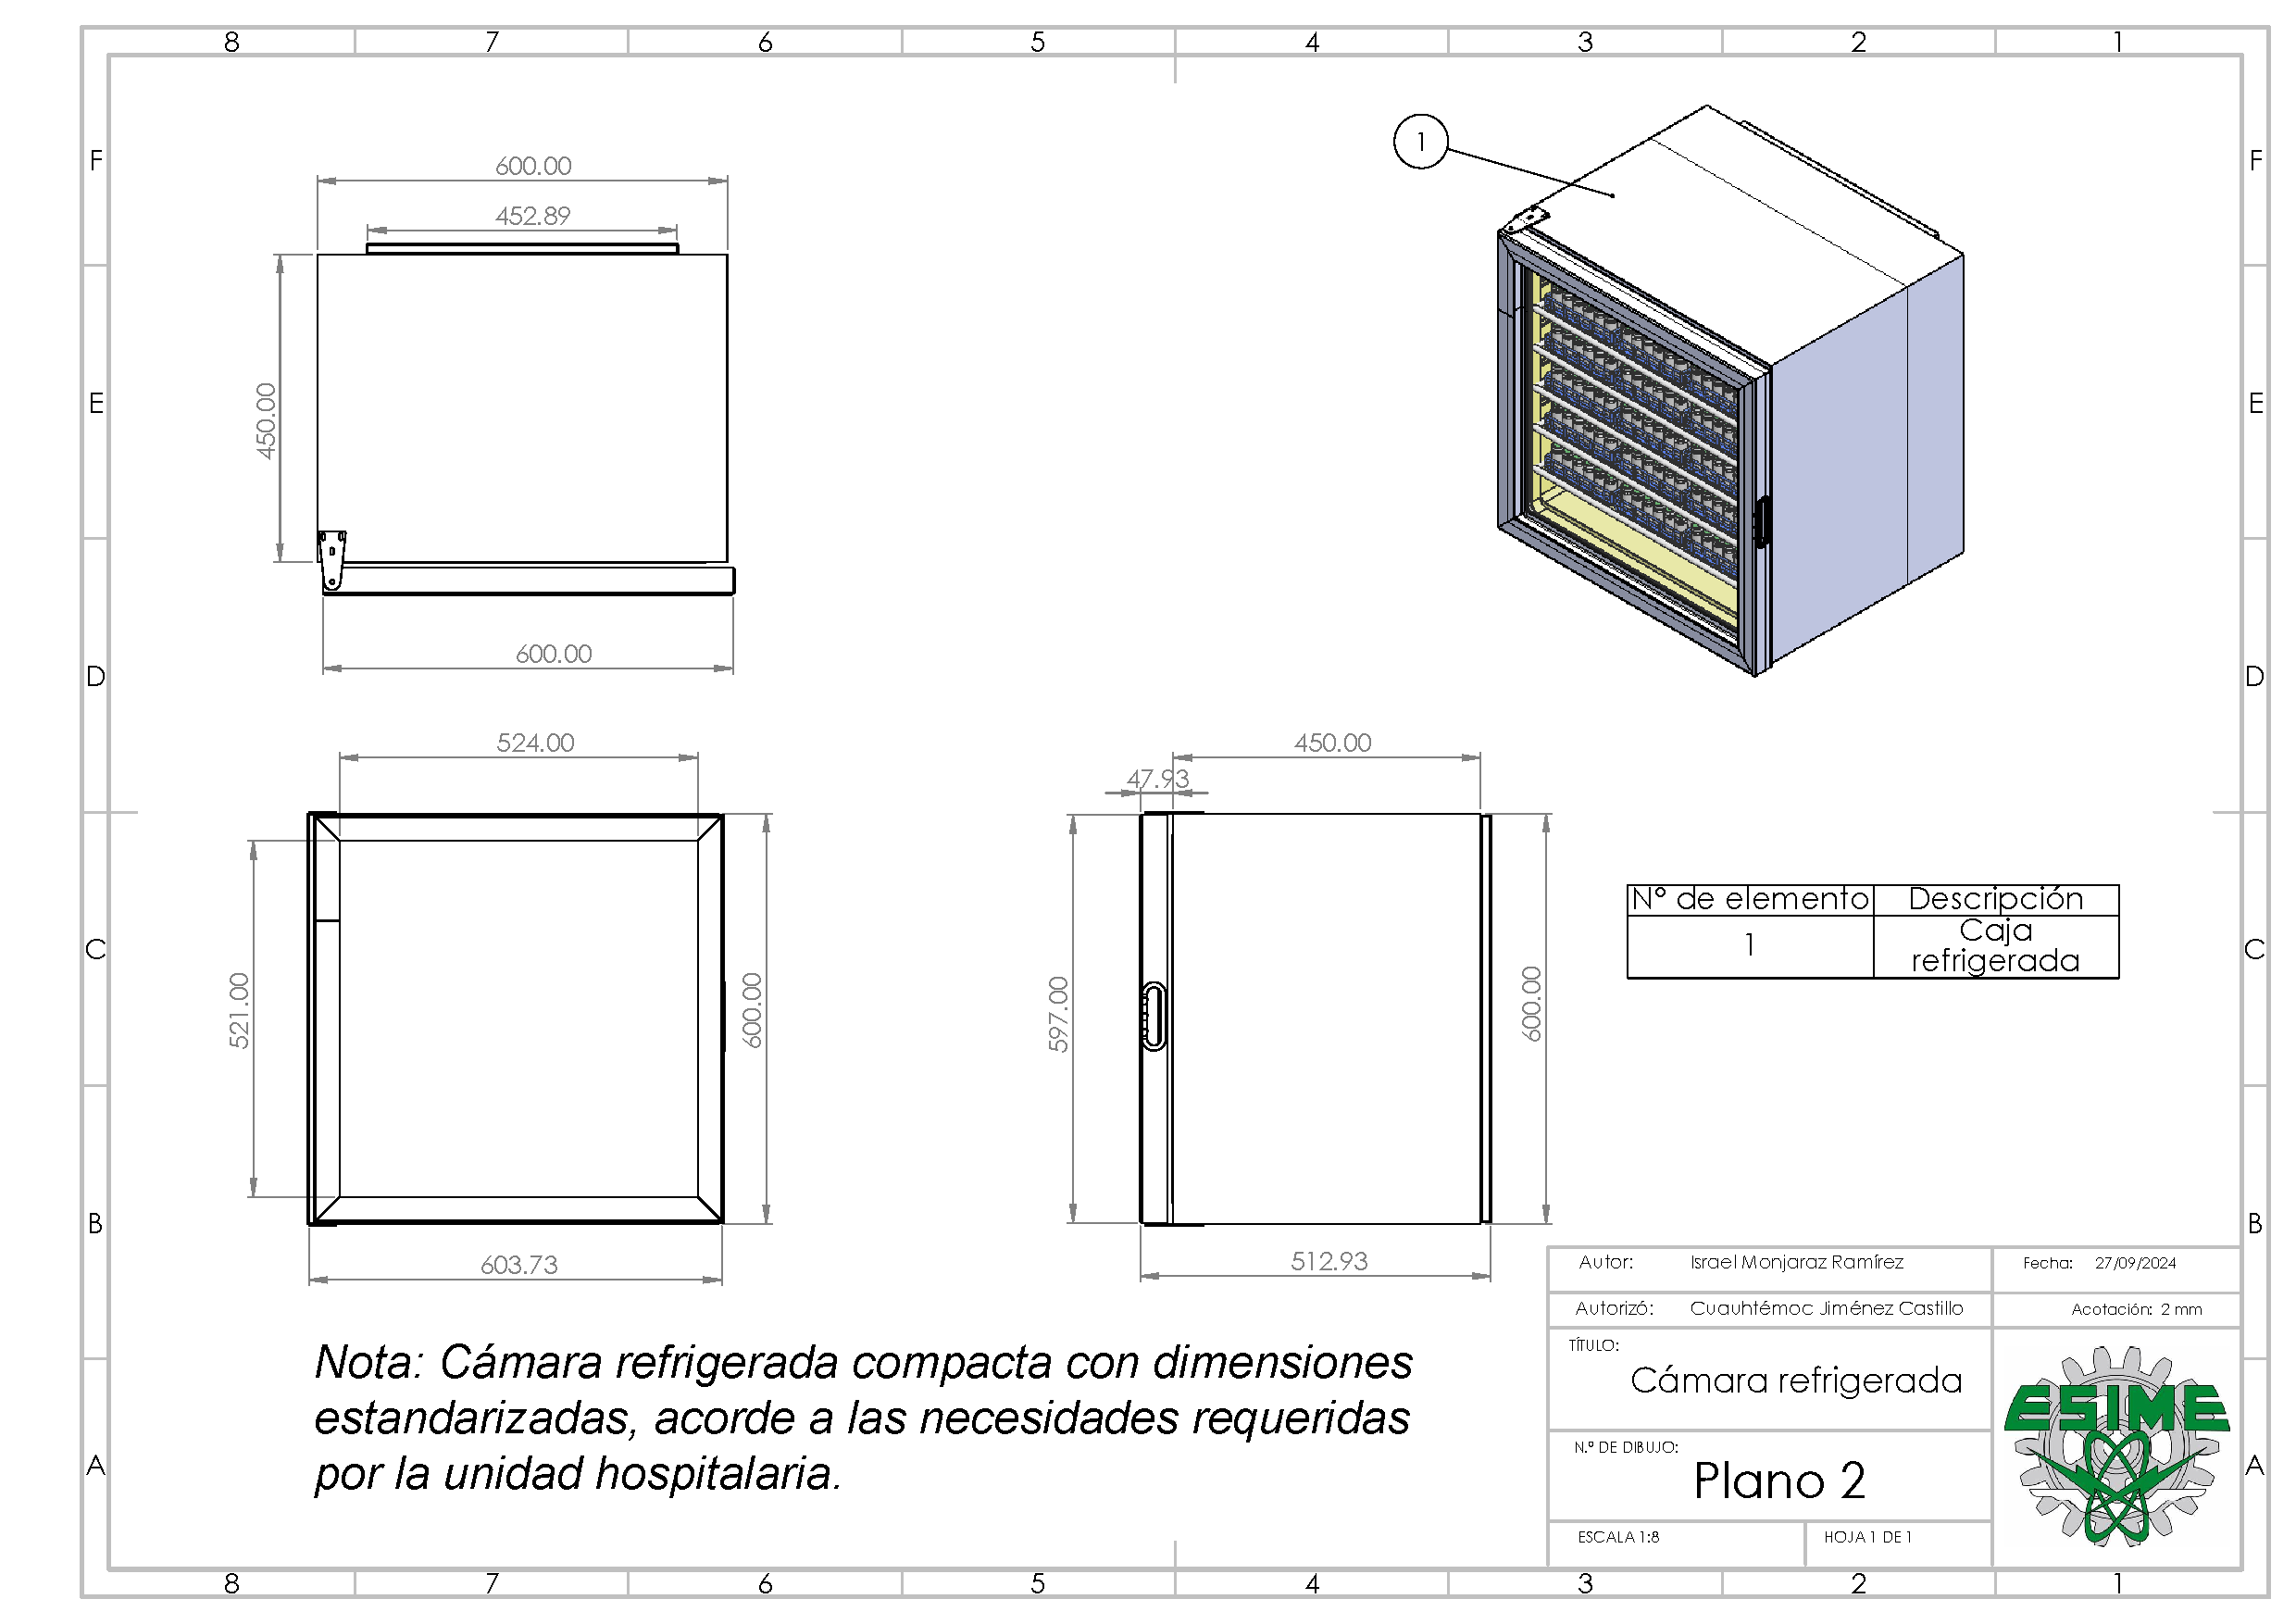
\includepdf[scale=0.75, angle=90]{pdfs/vistas-camara.pdf}
		\label{axo:vista-camara}
	\end{figure} 
\end{minipage}

\newpage
\section{Anexo 3. Diagrama eléctrico completo} 
\begin{minipage}{\textwidth} 
	\begin{figure}[H]
		\centering 
		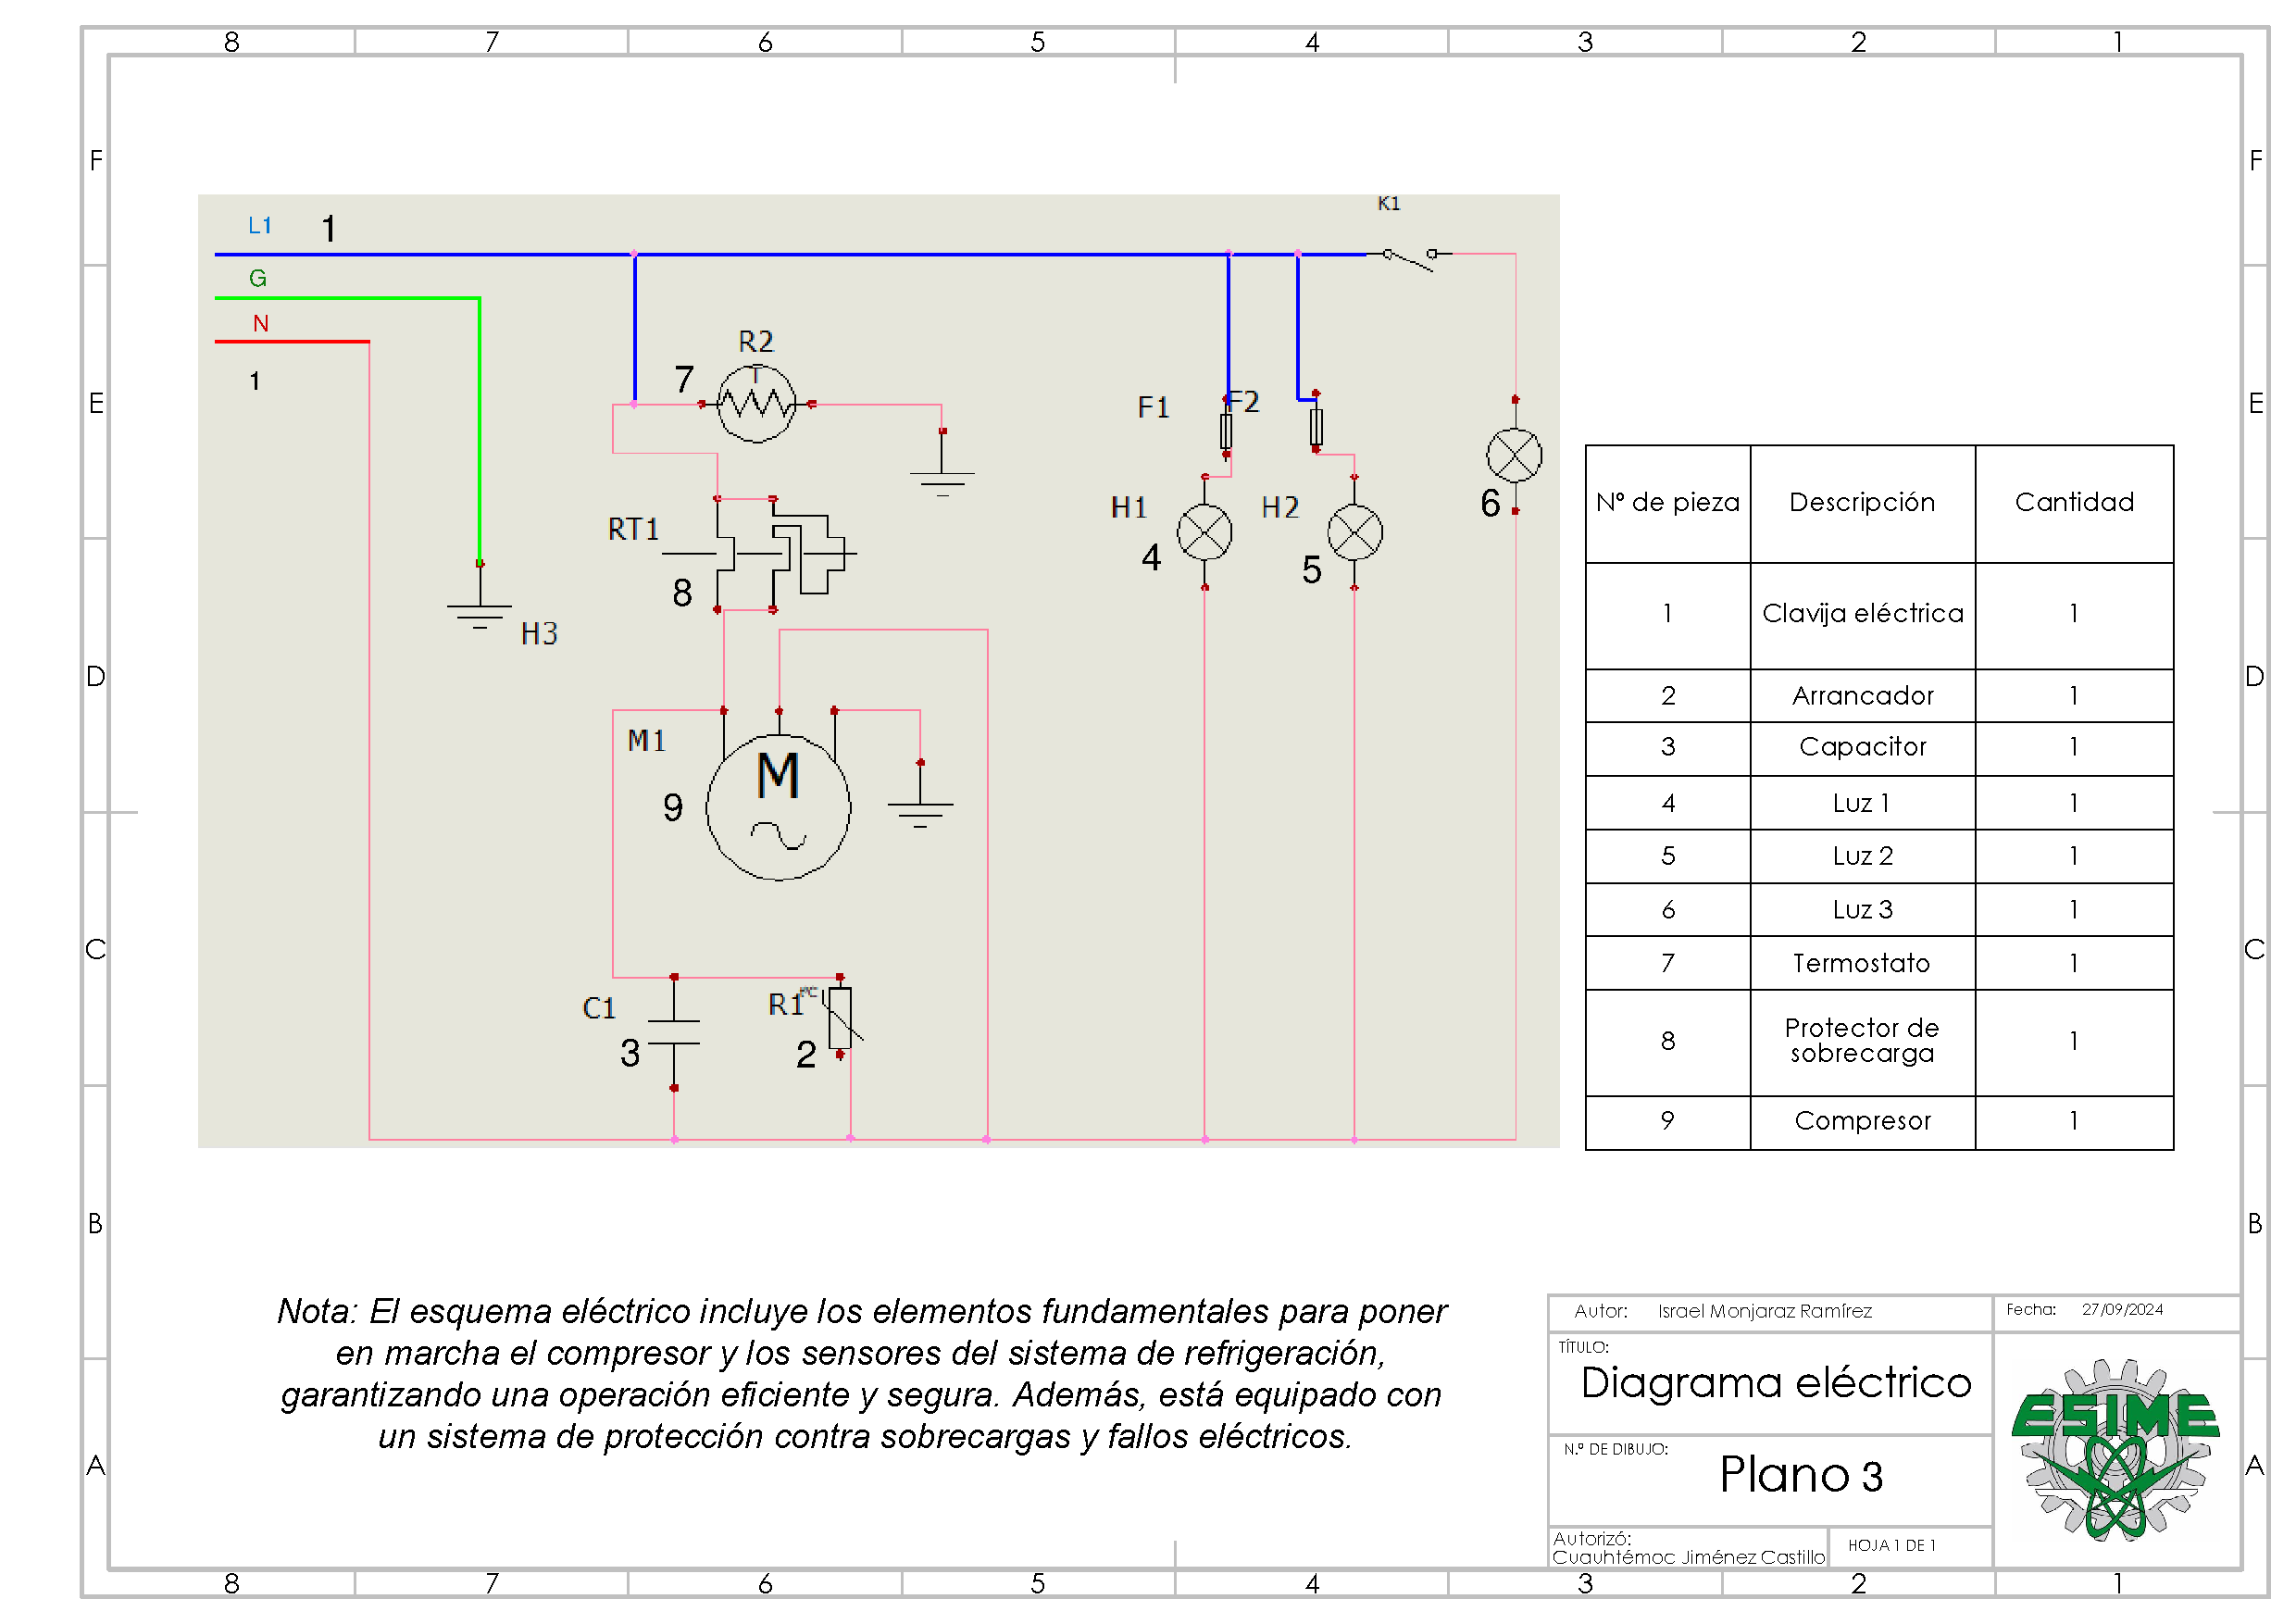
\includepdf[scale=0.75, angle=90]{pdfs/plano-electrico.pdf}
		\label{axo:diag-electrico}
	\end{figure} 
\end{minipage}

 




\newpage
\begin{minipage}{\textwidth}
	\section*{Tablas}
	\addcontentsline{toc}{section}{{Tablas}}\rsp \rsp	 
		\begin{table}[H]
 \centering
 \caption*{Anexo 4. Requerimientos y propiedades de almacenamiento para productos perecederos}\rsp\rsp\rsp
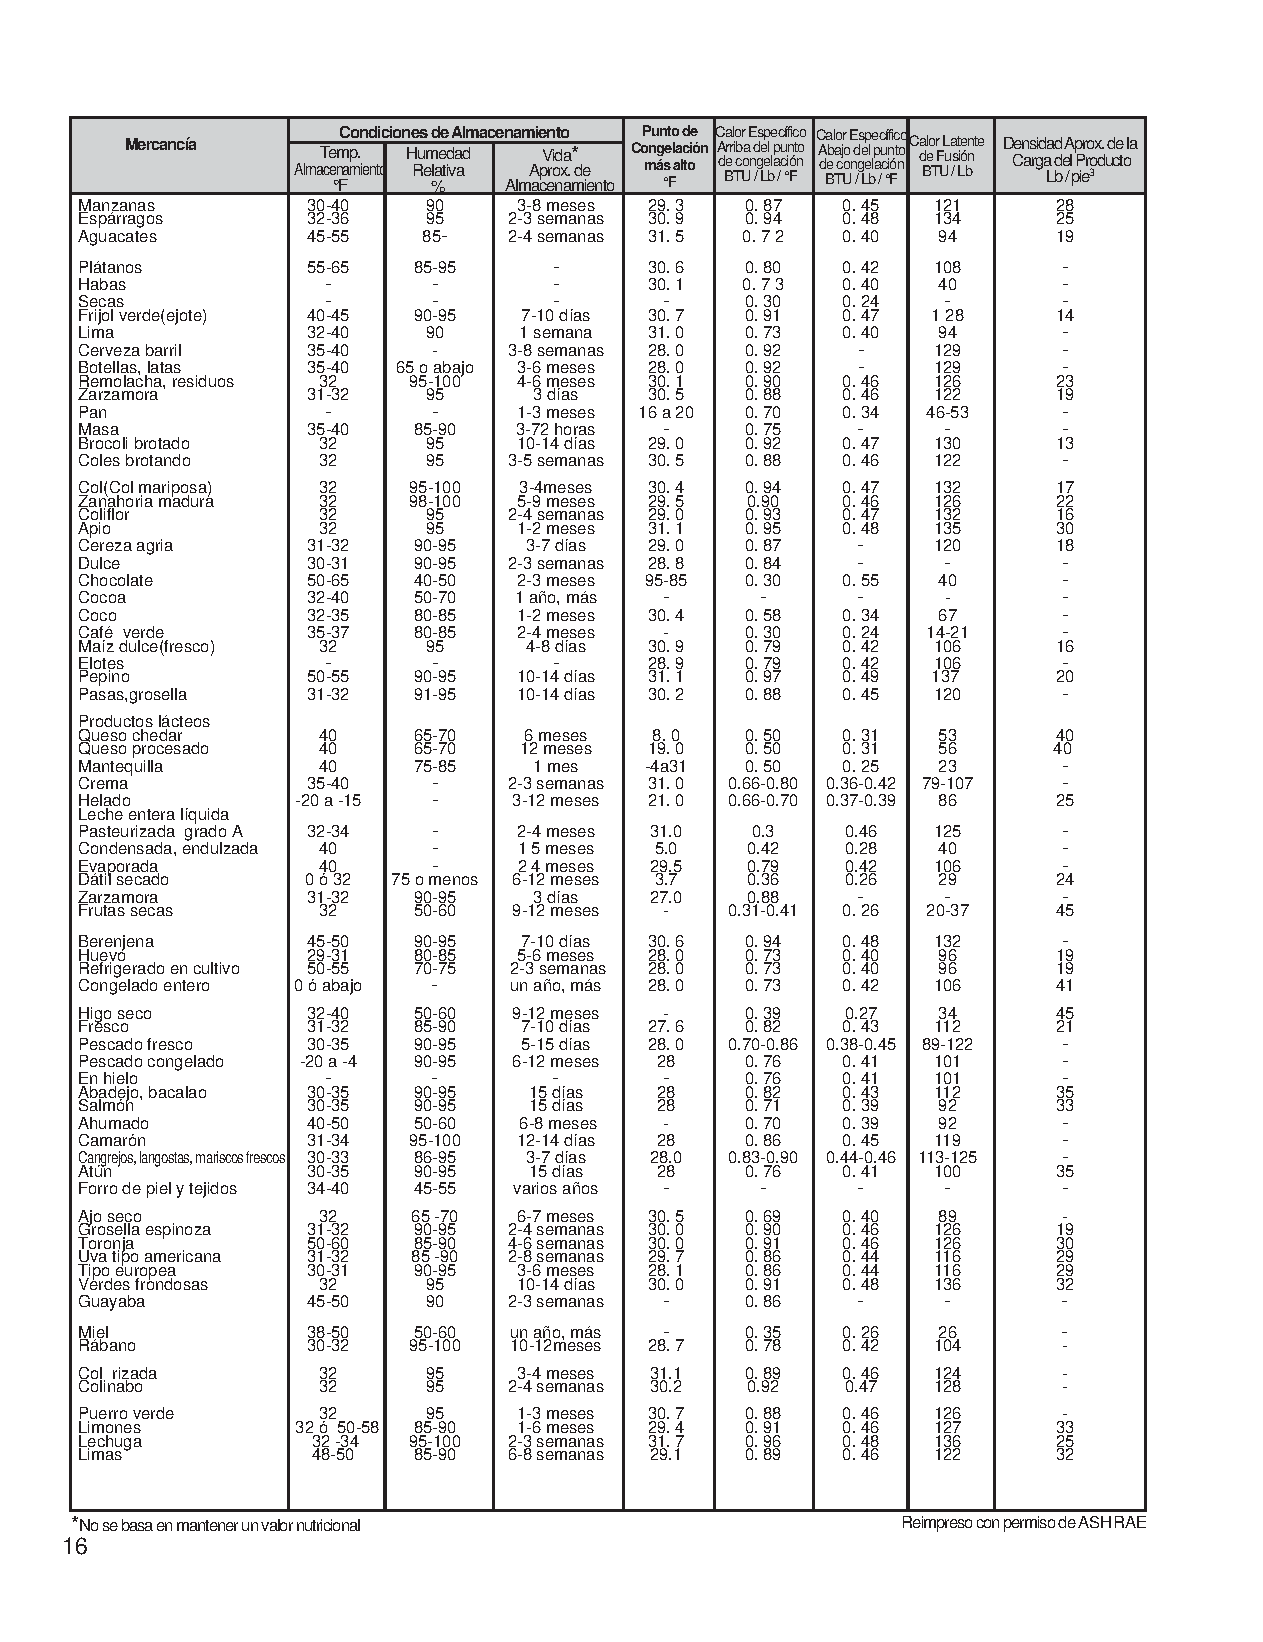
\includepdf[pages=1,scale=0.8]{bohn-perecederos.pdf}
 \label{anexo:bohn-perecederos}
		\end{table}		
	\end{minipage}
	
	
	 \newpage
	\begin{table}[H]
		\centering
		\caption*{\textit{Continuación de anexo 4.}}\rsp\rsp\rsp\rsp
		\includepdf[pages=2,scale=0.9]{bohn-perecederos.pdf}
		\label{anexo:bohn-perecederos2}
	\end{table}
	
	\newpage
	\section*{Imágenes}
		\addcontentsline{toc}{section}{{Imágenes}} 
	
	\begin{figure}[H]
		\centering
		%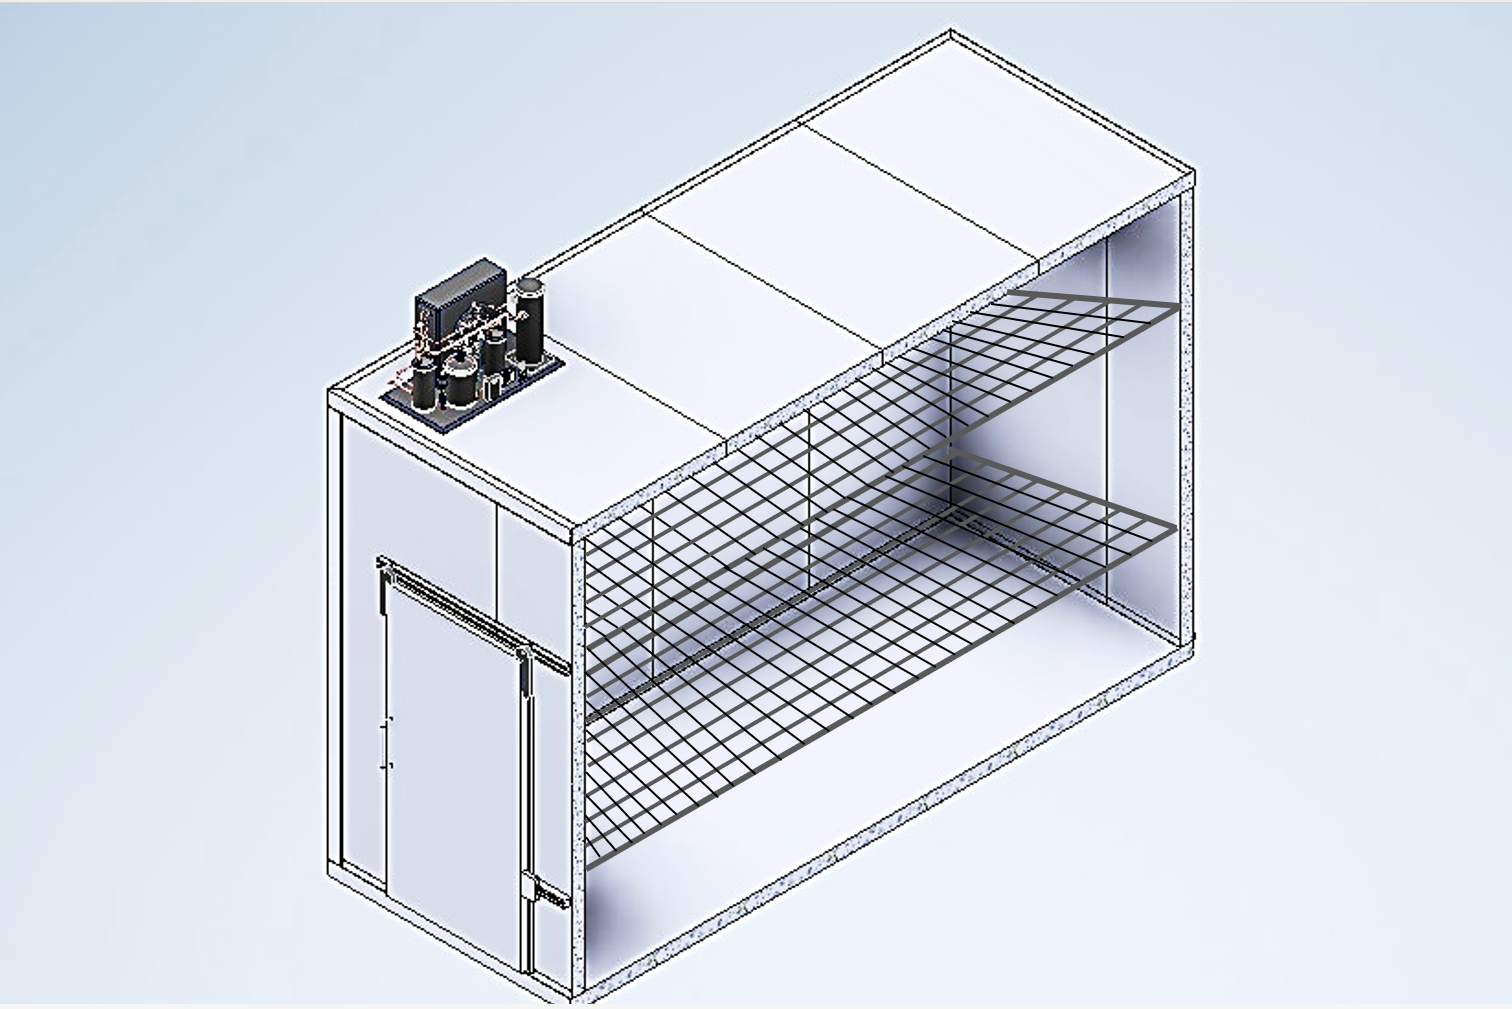
\includegraphics[width=0.6\linewidth]{figures/axo-design-div}
		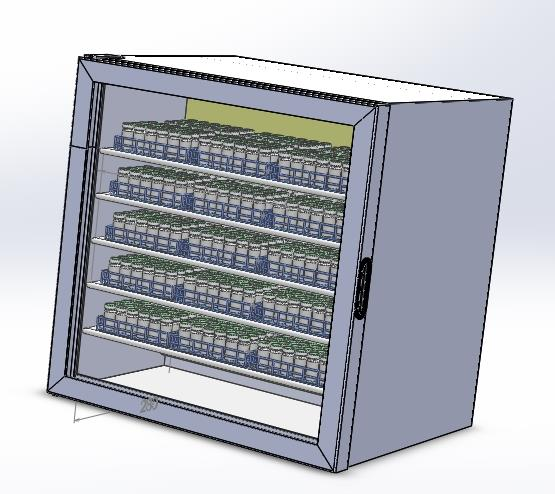
\includegraphics[width=0.415\linewidth]{figures/axo-parrilasycharolas}	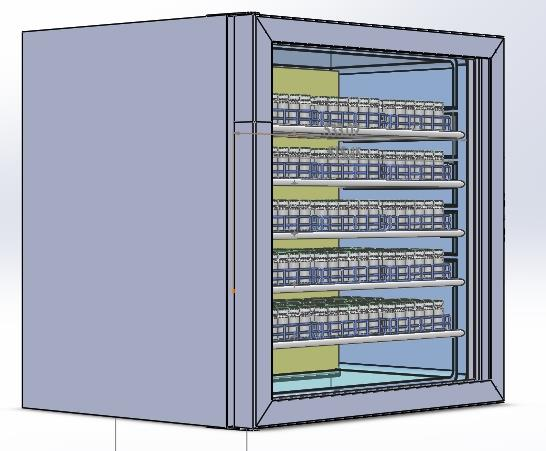
\includegraphics[width=0.415\linewidth]{figures/axo-parrilasycharolas2}
		\caption*{Anexo 5. Idea general de las divisiones al interior de la cámara.}
		\label{axo-design-div}
	\end{figure}
	
	 	\begin{figure}[H]
	 	\centering
	 	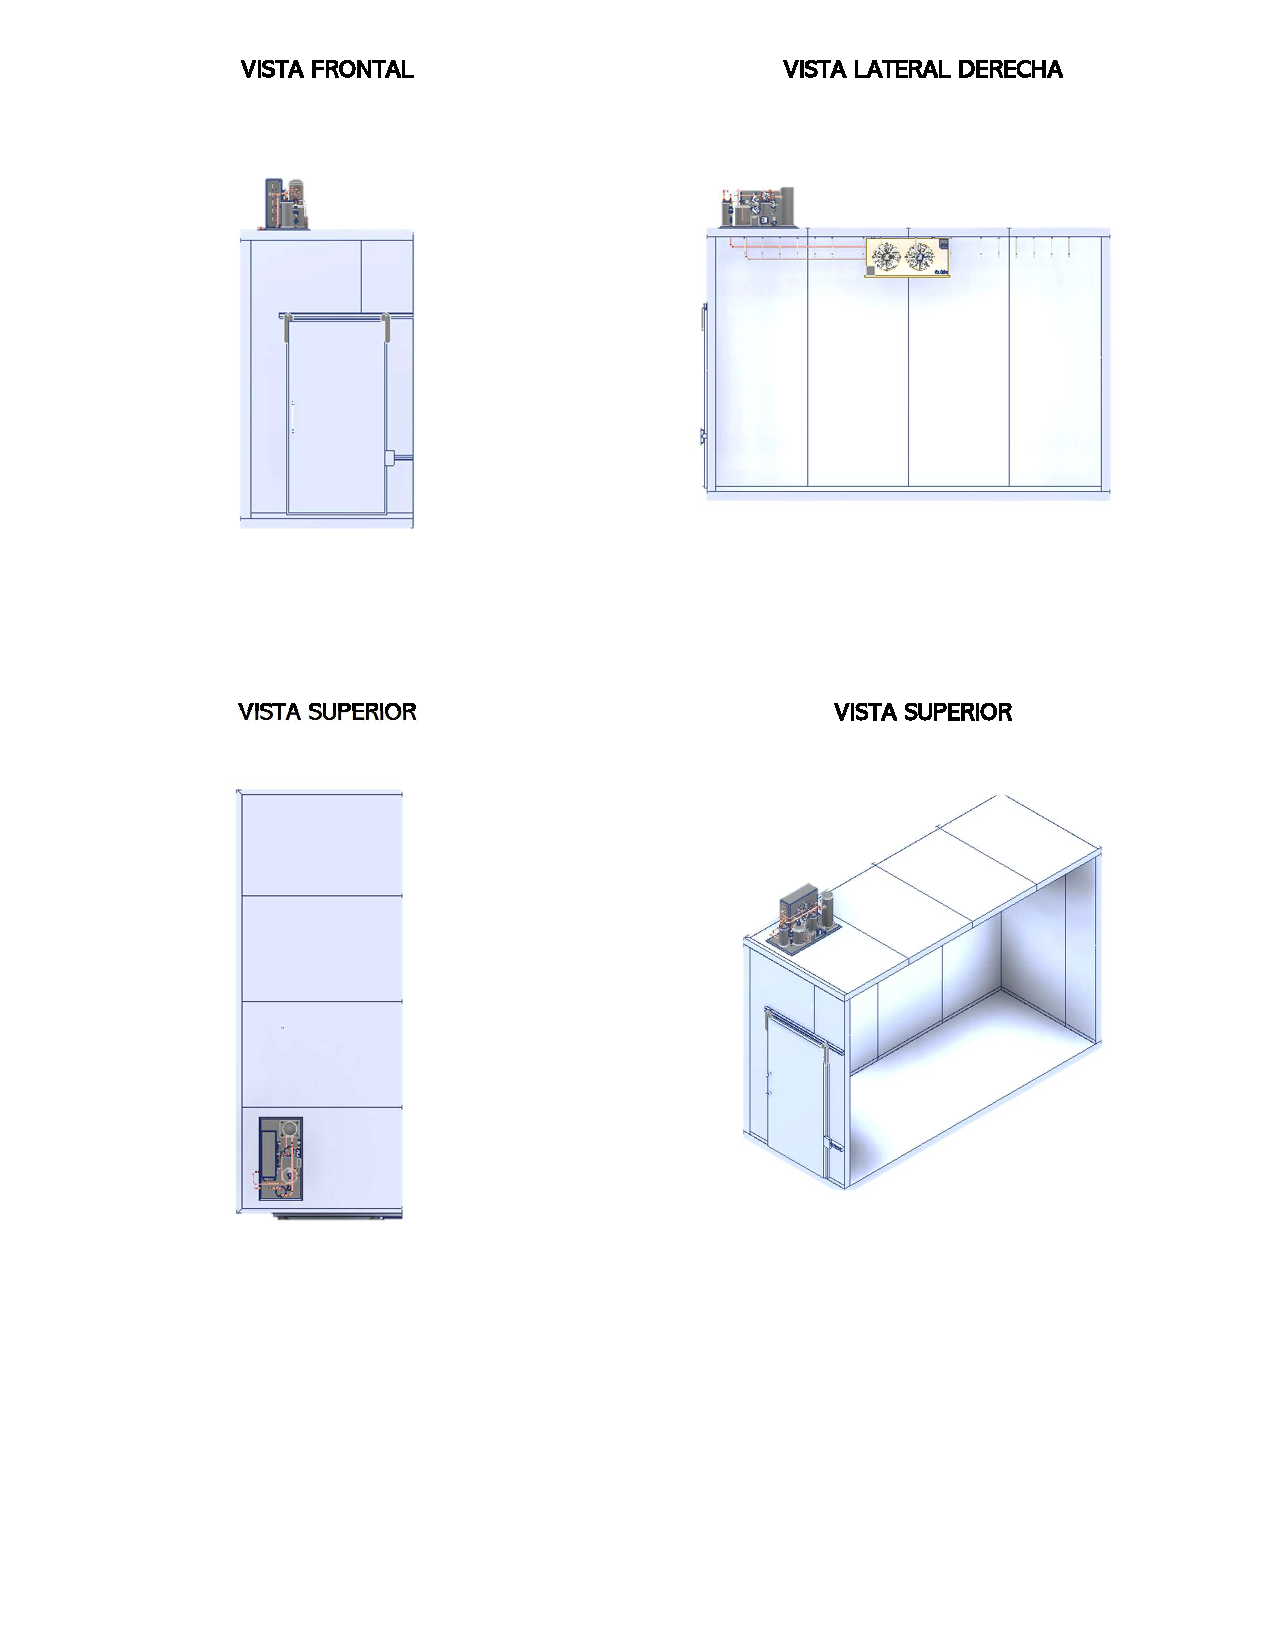
\includegraphics[width=0.7\linewidth]{figures/planos.pdf}
	 	\caption*{Anexo 6. Vistas de la cámara (diseño preliminar - capítulo 3).}
	 	\label{axo-planos}
	 \end{figure}
	 
 \begin{figure}[H]
 	\centering
 	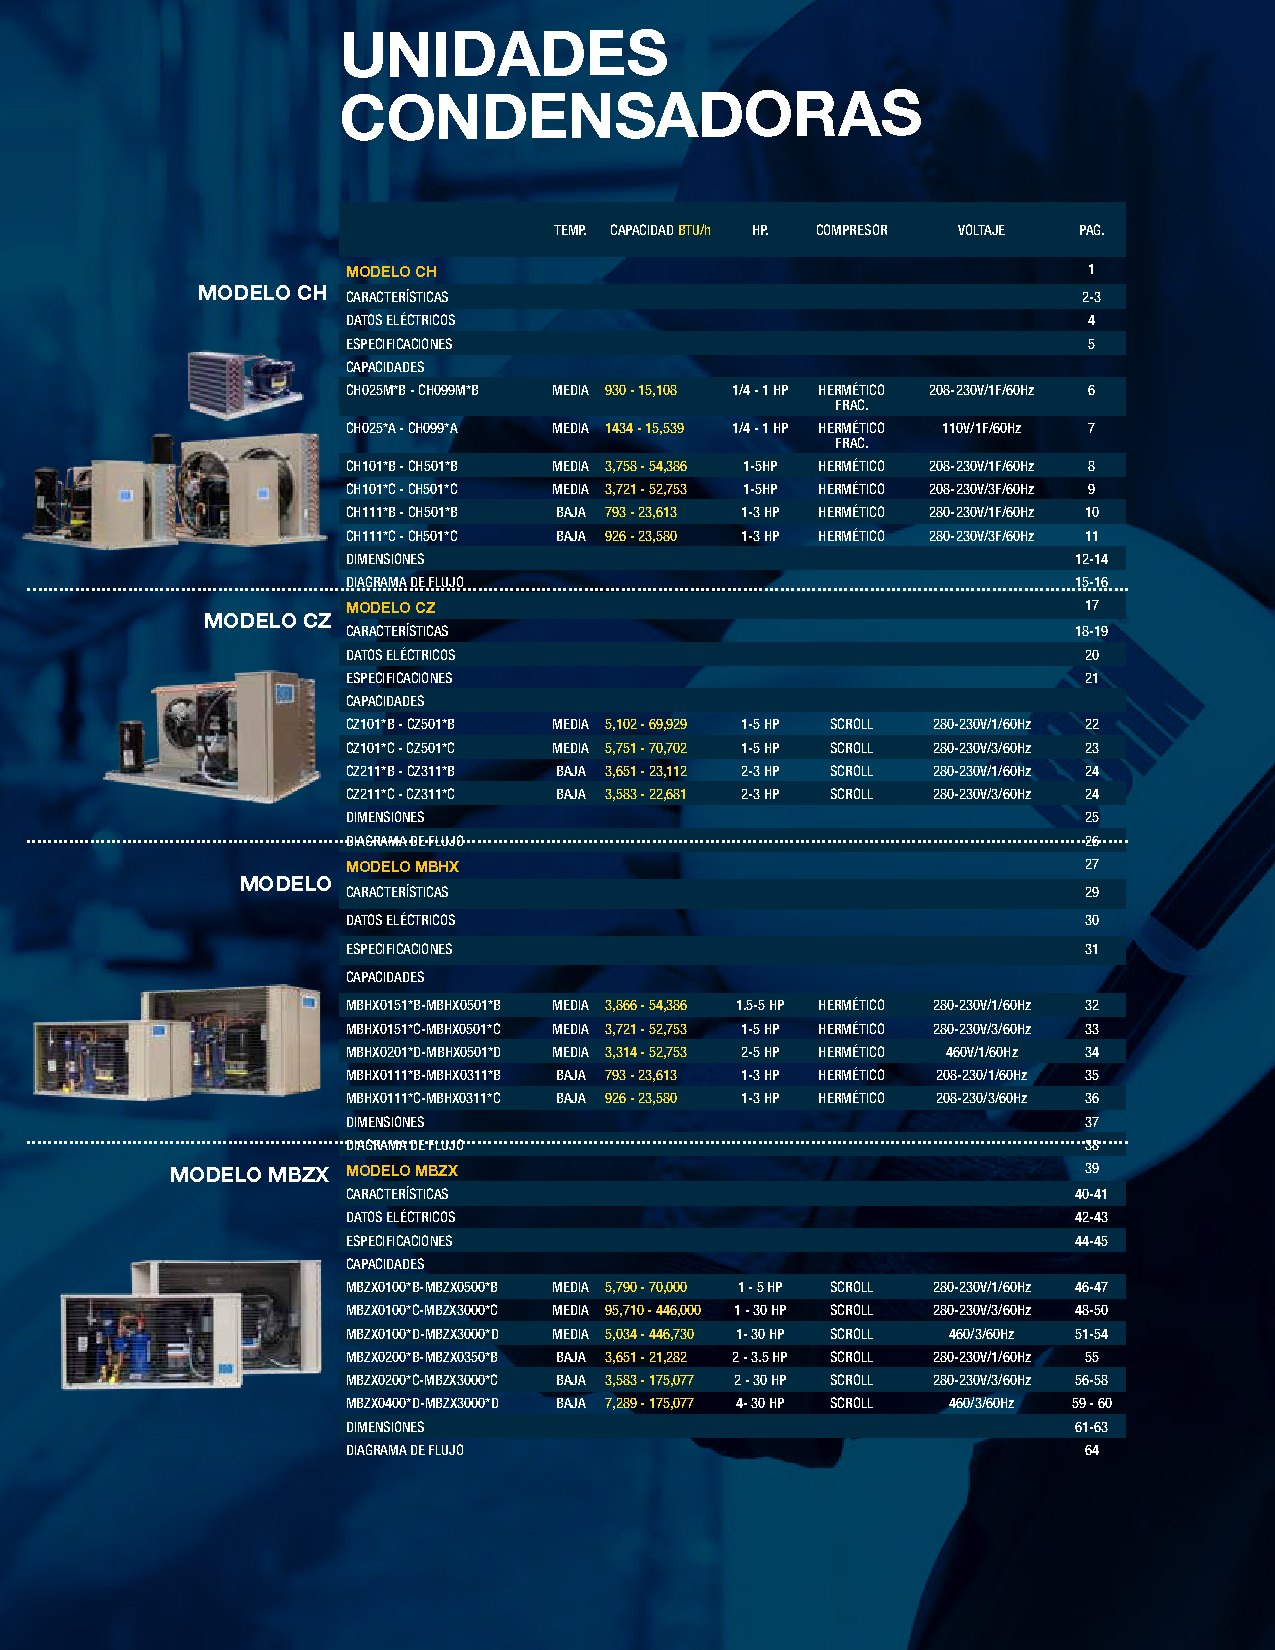
\includegraphics[width=0.8\linewidth]{figures/condensador-bohn}
	\caption*{Anexo 7. Manual Bohn para unidades condensadoras.}
 	\label{fig:axo-manual-thermo-king}
 \end{figure}
 
	 
	 